%%%% ijcai23.tex

\typeout{IJCAI--23 Instructions for Authors}

% These are the instructions for authors for IJCAI-23.

\documentclass{article}
\pdfpagewidth=8.5in
\pdfpageheight=11in

% The file ijcai23.sty is a copy from ijcai22.sty
% The file ijcai22.sty is NOT the same as previous years'
\usepackage{ijcai23}

% Use the postscript times font!
\usepackage{times}
\usepackage{soul}
\usepackage{url}
\usepackage[hidelinks]{hyperref}
\usepackage[utf8]{inputenc}
\usepackage[small]{caption}
\usepackage{graphicx}
\usepackage{amsmath}
\usepackage{amsthm}
\usepackage{booktabs}
\usepackage{algorithm}
\usepackage{algorithmic}
\usepackage[switch]{lineno}
% \usepackage{jmlr2e}
\usepackage{xcolor}
% \usepackage{caption}
\usepackage{subcaption}
\usepackage{amssymb}
\usepackage{multirow}
% \usepackage{tabularx}
% \usepackage{printlen}
\usepackage[T1]{fontenc}
\usepackage{dblfloatfix}
\usepackage{array,booktabs,ragged2e}

\newcolumntype{R}[1]{>{\RaggedLeft\arraybackslash}p{#1}}
\newsavebox{\imagebox}

% Comment out this line in the camera-ready submission
\linenumbers

\urlstyle{same}

% the following package is optional:
%\usepackage{latexsym}

% See https://www.overleaf.com/learn/latex/theorems_and_proofs
% for a nice explanation of how to define new theorems, but keep
% in mind that the amsthm package is already included in this
% template and that you must *not* alter the styling.
\newtheorem{example}{Example}
\newtheorem{theorem}{Theorem}
\newtheorem{definition}{Definition}[section]
% Following comment is from ijcai97-submit.tex:
% The preparation of these files was supported by Schlumberger Palo Alto
% Research, AT\&T Bell Laboratories, and Morgan Kaufmann Publishers.
% Shirley Jowell, of Morgan Kaufmann Publishers, and Peter F.
% Patel-Schneider, of AT\&T Bell Laboratories collaborated on their
% preparation.

% These instructions can be modified and used in other conferences as long
% as credit to the authors and supporting agencies is retained, this notice
% is not changed, and further modification or reuse is not restricted.
% Neither Shirley Jowell nor Peter F. Patel-Schneider can be listed as
% contacts for providing assistance without their prior permission.

% To use for other conferences, change references to files and the
% conference appropriate and use other authors, contacts, publishers, and
% organizations.
% Also change the deadline and address for returning papers and the length and
% page charge instructions.
% Put where the files are available in the appropriate places.


% PDF Info Is REQUIRED.
% Please **do not** include Title and Author information
\pdfinfo{
/TemplateVersion (IJCAI.2023.0)
}

\title{Assessing Future Geo-spatial Distribution of High Winds Risk with Deep Learning}


% Single author syntax
\author{
    Anonymous
}

% % Multiple author syntax (remove the single-author syntax above and the \iffalse ... \fi here)
% \iffalse
% \author{
% First Author$^1$
% \and
% Second Author$^2$\and
% Third Author$^{2,3}$\And
% Fourth Author$^4$
% \affiliations
% $^1$First Affiliation\\
% $^2$Second Affiliation\\
% $^3$Third Affiliation\\
% $^4$Fourth Affiliation
% \emails
% \{first, second\}@example.com,
% third@other.example.com,
% fourth@example.com
% }
% \fi

\begin{document}

\maketitle

\begin{abstract}
Accurate assessment of extreme wind risk is critical for infrastructure planning, disaster preparedness, and climate adaptation, yet remains fundamentally limited by the sparse and non-uniform distribution of surface weather stations. Climate models provide global spatial coverage but systematically underestimate local wind extremes due to spatial averaging. We propose a deep learning framework that bridges this gap by training a convolutional neural network to predict the probability of a locally extreme wind event at any location on a global grid, using gridded CMIP6 climate fields as input and ground-truth labels derived from over 6{,}000 GSOD weather stations worldwide. The target is defined as a station-adaptive binary indicator: whether the maximum observed wind speed within a 28-day window exceeds a location-specific threshold calibrated to the 95th percentile of local wind climatology. Evaluated on a held-out test period (2023--2024), our model achieves an AUROC of 0.849 and Average Precision of 0.753 globally, with consistent performance across climatically diverse regions including Europe, Siberia, and sub-Saharan Africa. The trained model can be applied directly to CMIP6 future scenario projections, enabling global storm-risk maps at $1.125^\circ$ resolution up to the year 2100.
\end{abstract}

\section{Introduction}
\label{sec:intro}

Increased greenhouse gas emissions are driving rapid growth in the number and severity of extreme weather events, including wind storms, flash floods, and droughts, with severe economic and social consequences. More than 332 natural disasters with damage exceeding \$1 billion each have been registered in the U.S. since 1980, with the annual economic toll continuing to rise~\footnote{\url{https://www.ncei.noaa.gov/access/billions/}}.

Predicting extreme wind events is fundamentally challenging: it requires estimating the probability of a rare event at a specific location, yet the observational network of surface weather stations is both sparse and non-uniform. Station density reflects population and economic development rather than meteorological need, leaving vast regions---high-latitude Siberia, central Africa, oceanic islands---virtually unmonitored. This is illustrated in Figure~\ref{fig:stations_coverage}, which shows the global distribution of GSOD stations used in this study.

\begin{figure}[ht]
    \centering
    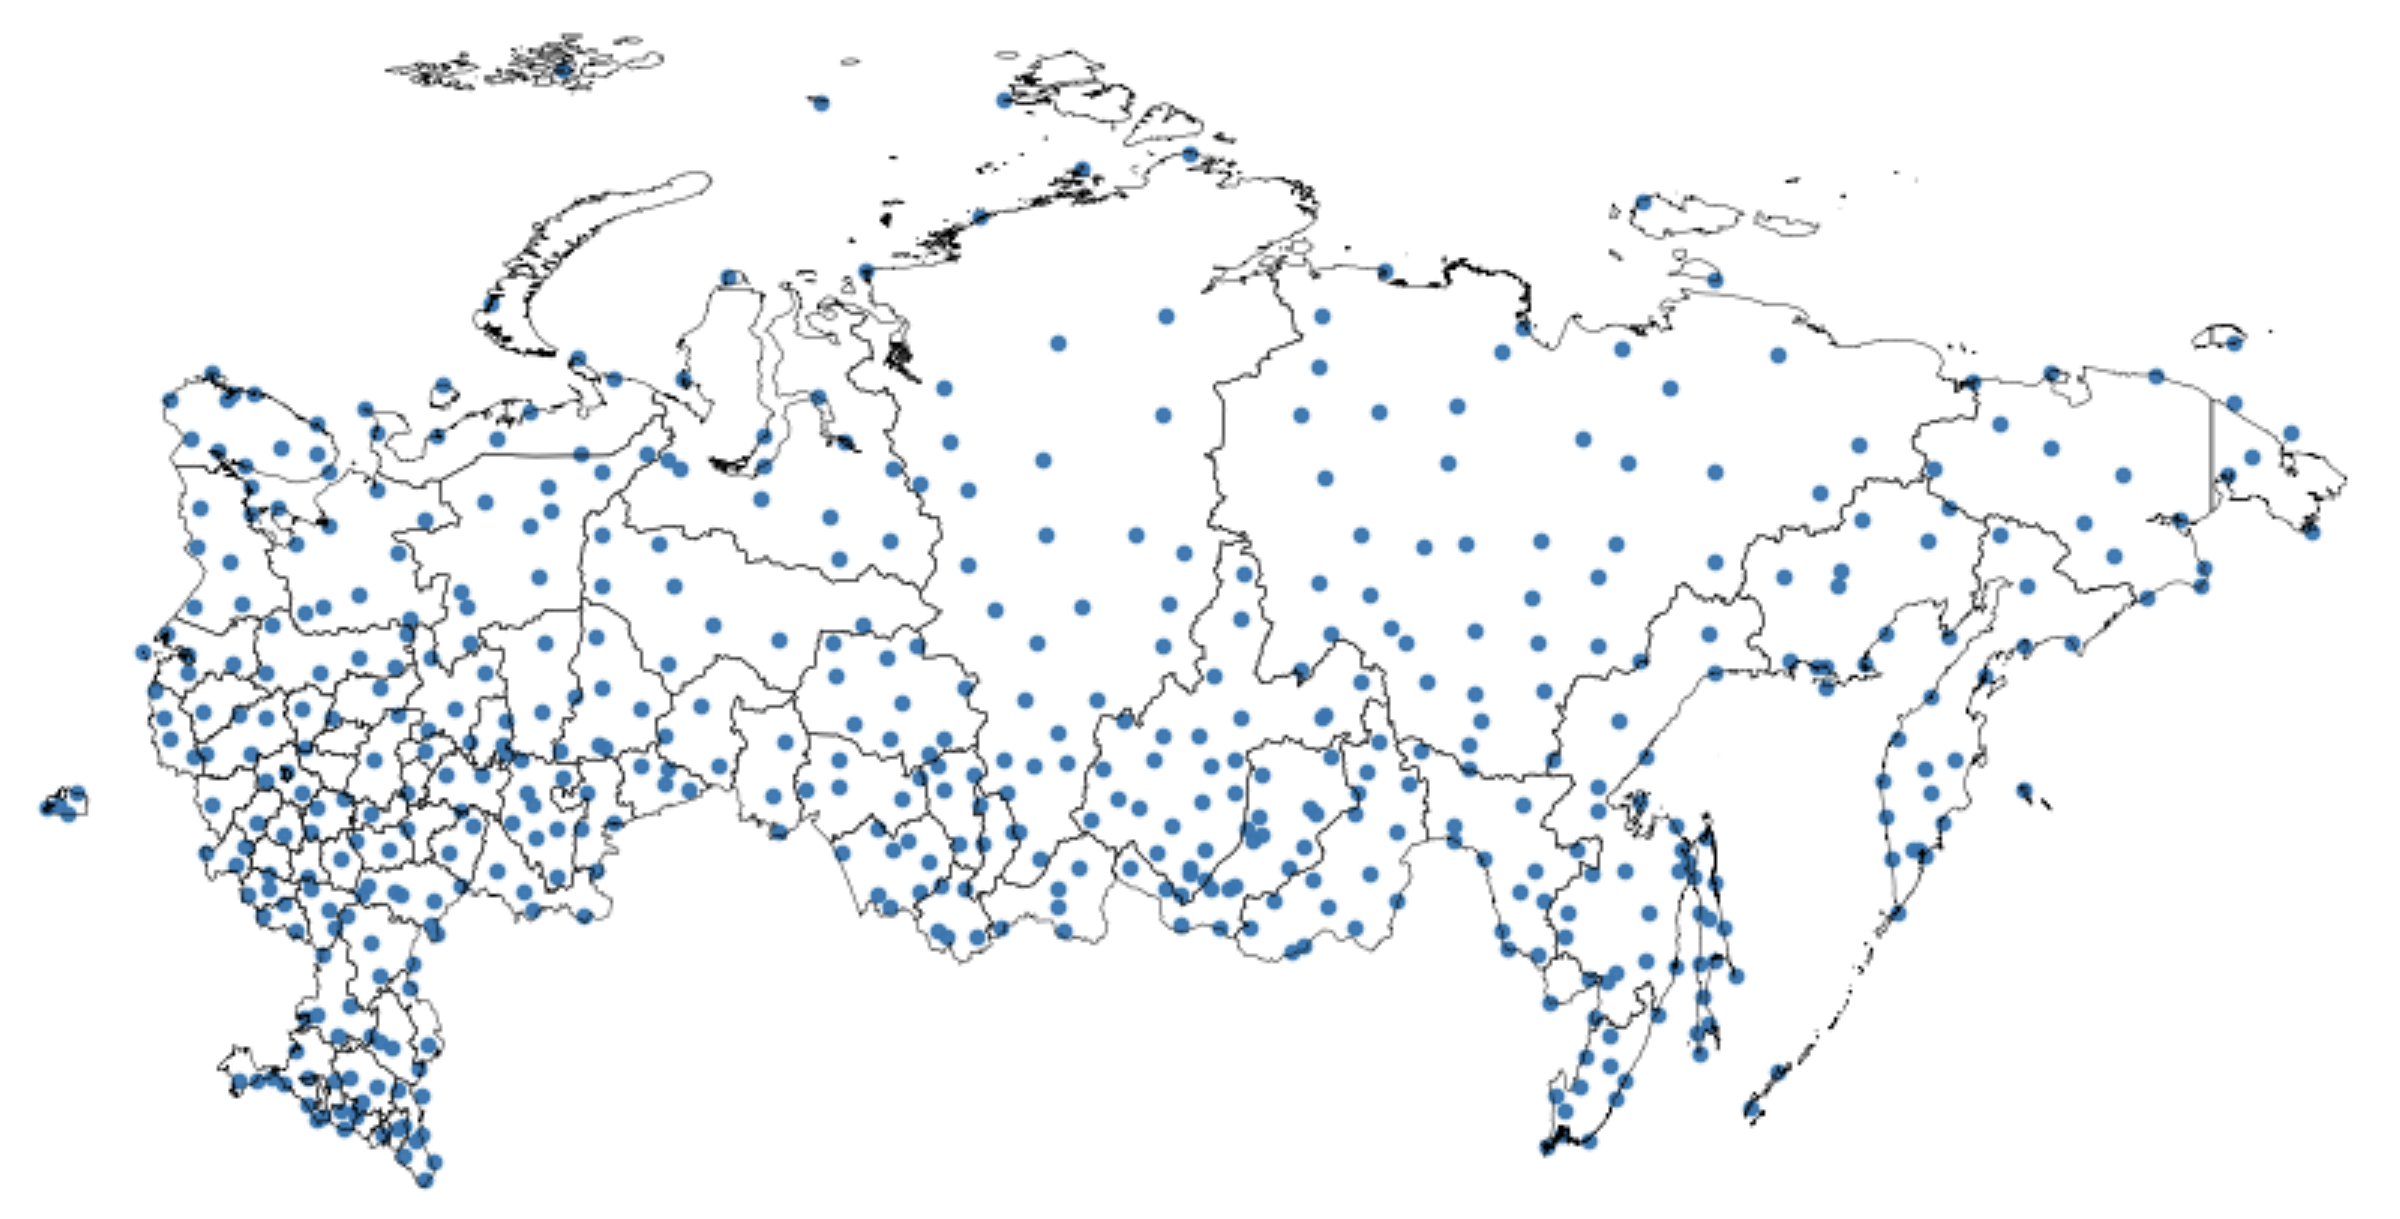
\includegraphics[width=\linewidth]{pics/stations_map.png}
    \caption{Global distribution of GSOD weather stations used in this study. Station density is highest over North America and Europe and sparse over central Africa, Siberia, and oceanic regions---a pattern representative of the data scarcity our method is designed to address.}
    \label{fig:stations_coverage}
\end{figure}

Climate models offer global spatial coverage but introduce a different limitation: by construction they represent grid-cell averages, systematically smoothing out the local extremes that drive damage. The sixth phase of the Coupled Model Intercomparison Project (CMIP6) provides daily fields on a $\sim$1$^\circ$ grid, capturing large-scale atmospheric dynamics but attenuating point-scale wind peaks by a factor of two or more relative to station observations~\cite{SILLMANN201765}.

We propose to bridge this gap with a data-driven calibration: a deep convolutional neural network (CNN) trained to predict, for each grid cell, the probability that the local wind speed will exceed a station-specific extreme threshold within a 28-day window, conditioned on the surrounding CMIP6 climate state. Once trained on historical data (2000--2022), the model can be driven by any CMIP6 scenario projection to produce global storm-risk maps up to 2100.

The contributions of this paper are threefold.
\begin{itemize}
    \item We introduce a station-adaptive target definition that combines a 28-day temporal aggregation window with a per-station 95th-percentile threshold, making the binary label both physically interpretable and robust across climatically heterogeneous regions (Section~\ref{sec:methodology}).
    \item We train and evaluate a global CNN model on over 6{,}000 GSOD stations worldwide, achieving an AUROC of 0.849 and Average Precision of 0.753 on a held-out 2023--2024 test period and demonstrating consistent performance across eight climatically distinct regions (Section~\ref{sec:experiments}).
    \item We conduct an ablation study isolating the contribution of each input variable (elevation, precipitation, temperature), and compare against two interpretable baselines derived from raw CMIP6 fields (Section~\ref{sec:experiments}).
\end{itemize}

This paper is organized as follows: Section~\ref{sec:rel_work} reviews related work on statistical downscaling and deep learning for climate extremes; Section~\ref{sec:methodology} describes the data, target definition, and model architecture; Section~\ref{sec:experiments} presents experimental results; Section~\ref{sec:conclusion} concludes with limitations and future directions.
\raggedbottom

\section{Related Work}
\label{sec:rel_work}

\paragraph{Classical statistical approaches to wind extremes.}
The traditional approach to extreme wind analysis fits Generalized Extreme Value (GEV) distributions to annual maxima or applies peaks-over-threshold (POT) methods. \cite{shang2021functional} propose fitting a GEV for each calendar day to estimate tail probabilities and mean extreme values. \cite{xiao2006probability} and \cite{liu2019long} analyse GEV families and return-period estimation for wind speed in specific regions. At the climate-model scale, \cite{kharinCMIP5GEV2013} evaluate 20-year return values for temperature and precipitation extremes in the CMIP5 ensemble using GEV distributions, while \cite{sillmannCMIP5extremes2013} benchmark CMIP5 models against 27 ETCCDI percentile-based extremes indices, providing the canonical non-ML baseline for exceedance-rate prediction. \cite{outtenSobolowski2021} apply POT to a 15-member Euro-CORDEX ensemble to project future extreme wind changes over Europe. While statistically principled, these methods require long local records, cannot extrapolate to unmonitored grid cells, and do not exploit the rich spatial context of surrounding climate fields.

\paragraph{Deep learning for extreme event detection from gridded data.}
The use of CNNs for extreme weather pattern recognition in gridded climate model output was pioneered by \cite{racahExtremeWeather2017}, who introduced a multichannel spatiotemporal CNN for semi-supervised detection of tropical cyclones and atmospheric rivers in CAM5 output, and by \cite{kashinathClimateNet2021}, who provided expert-labeled segmentation masks for the same task using a CGNet architecture. \cite{liu2016application} demonstrated CNN-based tropical cyclone detection from ERA5. \cite{reichsteinNature2019} provide the broader scientific framing: CNNs operating on spatiotemporal gridded data offer transformative potential for Earth system science. \cite{molinaBenchmark2021} established benchmark protocols for testing generalization of DL storm classifiers to future climate conditions, an aspect directly relevant to our CMIP6-trained model. The ExtremeWeather dataset \cite{racahExtremeWeather2017} and WeatherBench \cite{raspWeatherBench2020} provide community baselines for CNN-based extreme event detection and wind speed forecasting from gridded atmospheric fields, respectively.

\paragraph{Statistical downscaling and bias correction of climate models.}
Statistical downscaling trains a statistical or ML model to map coarse climate model output to fine-scale observations, directly analogous to our task of mapping CMIP6 grid cells to station-level extreme probabilities. \cite{banomedinaDeepESD2022} introduced DeepESD, a CNN-based perfect-prognosis downscaler for the CMIP5 multi-model ensemble, demonstrating that spatial convolutional architectures substantially outperform traditional regression-based methods. \cite{busterSRDRN2024} extend this with a super-resolution deep residual network combined with quantile delta mapping to simultaneously bias-correct and downscale six CMIP6 variables including surface wind over CONUS, addressing non-stationarity critical for future projections. \cite{harderConstrainedDL2023} introduce hard physical constraints (conservation-law renormalization layers) into CNN downscaling, improving out-of-sample accuracy. \cite{shenCMIP6Wind2022} quantify global CMIP6 systematic wind biases, showing that raw CMIP6 magnitudes systematically underestimate local extremes -- the core motivation for a learned calibration layer. \cite{gonzalez2020calibration} calibrate ERA5 wind using building-mounted sensors via quantile matching and random forests, showing that local corrections substantially improve agreement with point observations.

\paragraph{Probabilistic forecasting of wind extremes.}
\cite{schulzLerchWindGusts2022} conduct the most comprehensive comparison to date of ML methods for probabilistic wind gust forecasting at surface stations, including distributional regression networks (DRN), gradient-boosted EMOS, and quantile regression forests, on 175 German stations using a convection-permitting ensemble (COSMO-D2-EPS); the DRN achieves state-of-the-art skill. \cite{raspLerch2018} demonstrated that neural networks with station-specific embeddings outperform parametric EMOS for ensemble postprocessing, a design principle directly relevant to our station-adaptive threshold. \cite{lledo2020predicting} combine the S2S sub-seasonal forecast database~\cite{vitart2017subseasonal} with the Madden--Julian Oscillation phase to improve medium-range wind forecasts over Europe--Atlantic. These approaches post-process existing forecasts at individual stations or on a fixed grid, but do not produce spatially complete risk maps applicable to unobserved locations under future climate projections.

\paragraph{CMIP6 for wind impact assessment.}
Several recent studies use CMIP6 for downstream wind impact modelling. \cite{zhangBiGRUWind2021} train a BiGRU network to downscale CMIP6 near-surface wind speed to 0.25$^\circ$ for offshore wind resource projections in China to 2100. \cite{sorianoCMIP6offshore2023} combine bias-corrected CMIP6 wind projections with percentile-based classification of offshore wind energy adequacy along the Spanish coast -- one of the few papers applying a classification (rather than regression) framework to CMIP6 wind, making it a direct methodological comparator. \cite{krishnanCMIP6wind2020} show that CMIP6 improves over CMIP5 for Bay of Bengal near-surface wind but systematic biases remain, justifying our station-adaptive threshold design. \cite{zappaCORDEX2024} train an ML emulator on CMIP5-CORDEX simulations and transfer it to CMIP6 for wind energy drought projections, demonstrating that ML-based climate downscaling can bridge CMIP generations.

In summary, the existing literature addresses the component pieces of our problem -- GEV-based extreme analysis, CNN classification of extreme events from gridded data, statistical downscaling of climate model output -- but no prior work combines all three: a global, station-validated, binary extreme wind classifier trained end-to-end on CMIP6 fields with a station-adaptive target and evaluated on a held-out future period.


\section{Approach}
\label{sec:methodology}

This section outlines our approach, including problem setup, data collection and processing, algorithmic model, training, and classification.

\paragraph {Objective function.} The study focuses on assessing high wind risk and its consequences. To this end, according to the Beaufort wind damage scale, we focus on predicting the wind exceeding 20 meters per second, as it is considered dangerous. 

\paragraph {Classifier.} As the wind distribution is known to have a high spatial correlation, we employ a deep learning architecture specifically designed to capture such spatial dependencies. The specific architecture of our model is detailed in Section~\ref{sec:Deep_CNN}.

\begin{table*}[t]
    \centering
    \begin{tabular}{p{3cm}|p{4.7cm}|R{2.1cm}|R{2cm}|p{1.7cm}|p{1.6cm}} %  {c|c|c|c|c}
        \toprule
        Dataset Name & Bands cover & Time coverage & Spatial resolution, degree & Temporal resolution & Type  \\
        \midrule
        CMIP6 MRI-ESM2-0 \cite{SeijiYukimoto20122012-A02} & Daily max.\ wind speed, precipitation, max.\ and min.\ temperature & $1850 - 2100$ & $1.125$ &  Day & Model \\
        \midrule
        GSOD weather stations \cite{gsod23}&  Temperature, air pressure, precipitation, wind speed, soil, solar radiation, drought index, cloudiness, extremes & $1929 - 2025$ & Discrete &  Day & Measured\\
        \midrule
        GLOBE \cite{hastings1998development} &  Elevation & - & $0.008$ &  - & 
        Digital Elevation Model (DEM) \\
        \bottomrule
    \end{tabular}
    \caption{Datasets used for modeling%{\color{red} in two column formatting that must be over both columns}
    }
    \label{tab:datasets}
\end{table*}

% \multirow[t]{3}{*}{Model}  \\
% \cmidrule{1-5}

\subsection{Data Collection and Preprocessing}
\label{sec:data_collection_preprocessing}

\paragraph{Data.}
To assemble the training dataset we combine a global climate reanalysis with ground-truth station measurements and a digital elevation model.

\textbf{Climate model.} We use the historical simulation of the Coupled Model Intercomparison Project Phase~6 (CMIP6) MRI-ESM2-0 model~\cite{SeijiYukimoto20122012-A02} as our primary climate input. CMIP6 provides daily gridded fields at a nominal resolution of $1.125^\circ \times 1.125^\circ$ ($\approx 125$~km at the equator) on a uniform global grid covering latitudes $90^\circ$S--$90^\circ$N and longitudes $0^\circ$--$360^\circ$. We use four surface variables: daily maximum near-surface wind speed (\texttt{sfcWindmax}), total precipitation (\texttt{pr}), daily maximum temperature (\texttt{tasmax}), and daily minimum temperature (\texttt{tasmin}). These variables were selected because they jointly capture the synoptic-scale thermodynamic and dynamic state that drives wind extremes: temperature gradients set baroclinic instability, precipitation indicates convective activity, and the model wind field provides a direct, if spatially smoothed, signal of the large-scale circulation.

\textbf{Station observations.} For ground-truth labels we use the Global Surface Summary of the Day (GSOD) dataset~\cite{gsod23}, which archives daily observations from over 9{,}000 weather stations worldwide covering the period 1929--present. After quality filtering (stations with fewer than 25 valid observations in any 6-month window are discarded, and stations with implausibly low or high wind climatology are excluded), our global training set retains approximately 6{,}045 stations distributed across all continents. The non-uniform spatial distribution of this observational network---densest over North America and Europe, sparser over Africa and Central Asia---is illustrated in Figure~\ref{fig:stations_coverage}.

\textbf{Digital Elevation Model.} To account for the influence of topography on local wind patterns, we incorporate the Global Land One-kilometer Base Elevation (GLOBE) dataset~\cite{hastings1998development} as an additional input channel. The GLOBE DEM is aggregated spatially to match the CMIP6 grid by computing the mean elevation within each target grid cell. Elevation acts as a static fifth input channel alongside the four time-varying CMIP6 variables.
%Data collection and preprocessing consist of several steps. First is obtaining the required climatic variable model of a region of interest, such as a state.{\color{blue} I do not understand. Which state?} The second is obtaining the real measurements for weather stations. 

%The following step matches the climate model pixels with the locations of weather stations both spatially and temporarily. {\color{blue} Please rewrite this. Unclear}

Table \ref{tab:datasets} summarizes the description of real (observational) and synthetic (model-based) datasets used in this study. Synthetic datasets cover each region uniformly, while the real ones often cover the most populated areas only. 
% Future projections of the synthetic datasets are based on various CO${}_2$ emission scenarios, critically reviewed in \cite{eyring2016overview}.


\begin{figure}[!b]
     \centering
     \captionsetup{justification=centering}
     \begin{subfigure}[b]{0.49\linewidth}
         \centering
         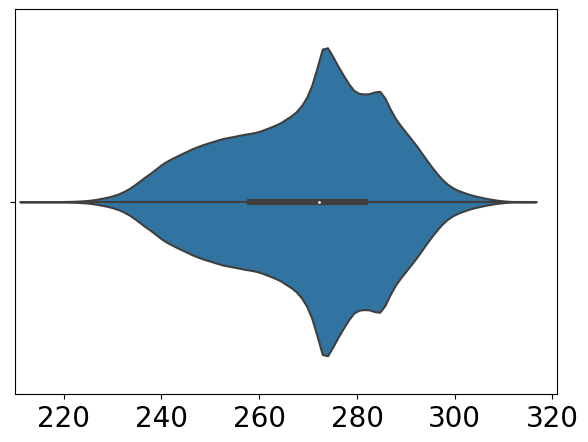
\includegraphics[height=3.3cm, width=\linewidth]{pics/cmip_temperature.png}
         \caption{CMIP6 MRI-ESM2-0 temperature, K}
         \label{fig:violins_data_era5_t}
     \end{subfigure}
     \hfill
     \begin{subfigure}[b]{0.49\linewidth}
         \centering
         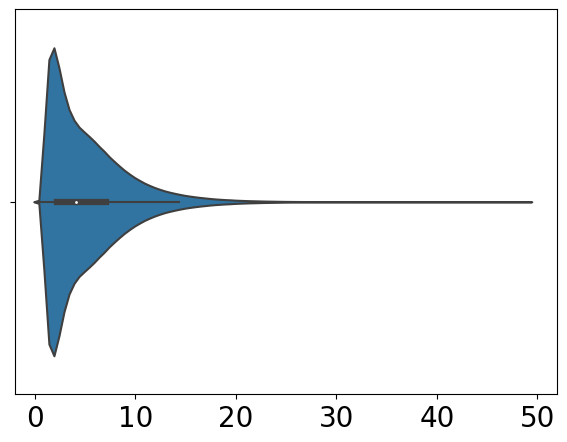
\includegraphics[height=3.3cm, width=\linewidth]{pics/cmip5_wind.png}
         \caption{CMIP6 MRI-ESM2-0 daily max.\ wind speed, m/s}
         \label{fig:violins_data_era5_ws}
     \end{subfigure}
     \hfill
     \\
     \begin{subfigure}[b]{0.49\linewidth}
         \centering
         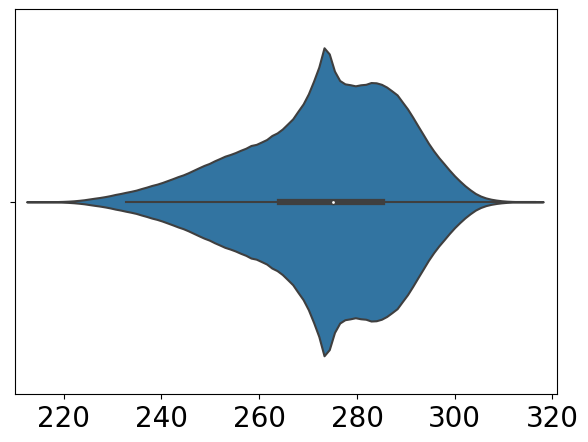
\includegraphics[height=3.3cm, width=\linewidth]{pics/stations_temperature2.png}
         \caption{Stations temperature, K}
         \label{fig:violins_data_ws_t}
     \end{subfigure}
     \begin{subfigure}[b]{0.49\linewidth}
         \centering
         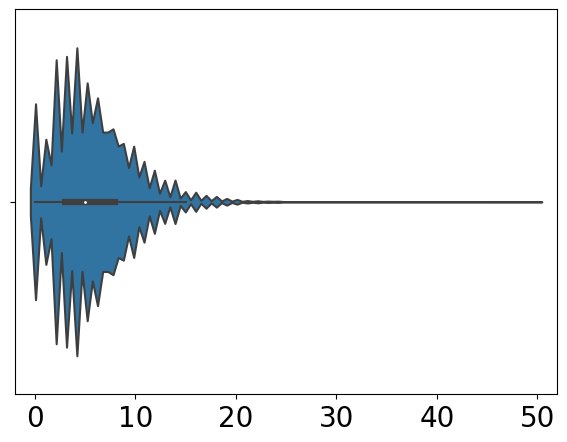
\includegraphics[height=3.3cm, width=\linewidth]{pics/stations_wind2.png}
         \caption{Stations wind speed, m/s}
         \label{fig:violins_data_ws_ws}
     \end{subfigure}
        \caption{Distribution of daily maximum temperature (a,\,c) and daily maximum near-surface wind speed (b,\,d) from the CMIP6 MRI-ESM2-0 climate model and GSOD station measurements, global training period (2000--2020). Boxes show the interquartile range; whiskers extend to the 5th--95th percentile. CMIP6 grid-cell averages capture the bulk distribution well but attenuate the extreme tails relative to point observations---the core bias our model is designed to correct.}
        \label{fig:violins_data}
\end{figure}

Figure~\ref{fig:violins_data} compares the distributions of temperature (a,~c) and daily maximum wind speed (b,~d) from the CMIP6 MRI-ESM2-0 model and GSOD station measurements over the global training period (2000--2022). The plots show strong agreement in the median, interquartile range, and overall shape for both variables. This concordance confirms that CMIP6 provides a suitable physical basis for training the predictive model, even though the model's grid-cell averages systematically attenuate the tails of the wind speed distribution relative to point observations---the core challenge our method addresses.

\begin{table}[!b]
    \centering
    \begin{tabular}{p{0.7cm}|p{4.1cm}|p{2.5cm}}%{c|c|c|c|c}
        \toprule
        Letter & Name & Domain  \\
        \midrule
        \multicolumn{3}{c}{Geophysical variables in a pixel} 
        \\
        \midrule
        $\mathcal{T}_{max}$ & Maximum temperature & $\mathbb{R}^3$   \\
        \midrule
        $\mathcal{T}_{min}$ & Minimum temperature & $\mathbb{R}^3$   \\
        \midrule
        $\mathcal{E}$ & Average elevation & $\mathbb{R}^2$   \\
        \midrule
        $\mathcal{P}$ & Total precipitation & $\mathbb{R}^3$   \\
        \midrule
        $\mathcal{WS}$ & Maximum wind speed & $\mathbb{R}^3$   \\
        \midrule
        \multicolumn{3}{c}{Miscellaneous}
        \\
        \midrule
        $\mathcal{S}$ & Set of weather stations & -
        \\
        \midrule
        $\tau$ & Wind speed threshold for target variable definition & $\mathbb{R}$ \\
        \midrule
        $w$ & Half of a pixel vicinity & $\mathbb{N}$
        \\
        \midrule
        $\mathcal{D}$ & Dataset of matched pixels of climatic variables $X$ and target values $Y$ &  
        $X\in\mathbb{R}^{C \times 2w \times 2w}$,
        $Y \in \{0, 1\}$
        \\
        \bottomrule
    \end{tabular}
    \caption{Notation}
    \label{tab:table_of_notations}
\end{table}

We use calligraphic letters to denote tensors of pixels that form the climate model. The notation is summarized in Table~\ref{tab:table_of_notations}. In all tensors, the first dimension indexes time (daily steps), the second indexes latitude (south to north), and the third indexes longitude (west to east). For example, $(\mathcal{WS})_{t,i,j}$ denotes the daily maximum near-surface wind speed on day $t$ at grid cell $(i,j)$.

The next crucial step is a resolution matching for geophysical tensors. Different datasets typically have different spatial and temporal resolutions outlined in Table \ref{tab:datasets}. To match the resolutions, we aggregate DEM data spatially to match the resolution of climate models. After aggregation, we retain the mean elevation within each CMIP6 grid cell. This scalar field is used as a static fifth input channel alongside the four time-varying CMIP6 variables, broadcast uniformly across the temporal dimension of each input patch (see Section~\ref{sec:Deep_CNN}).

A crucial preprocessing step is to standardize the spatial and temporal resolutions of all geophysical tensors, as they originate from different sources. 
For the spatial dimensions, we first define a target resolution and resample each tensor to match it. If a tensor's original resolution is higher than the target, we downsample by averaging the values within each target grid cell. Conversely, if the resolution is lower, we upsample using $2D$ cubic interpolation, as implemented in SciPy \cite{2020SciPy-NMeth}. 
For the temporal dimension, we aggregate data to a daily frequency by taking the maximum value, a choice motivated by our focus on extreme events. This alignment process ensures that all climate variables are represented on a consistent spatiotemporal grid, which is essential for the model.

\begin{example}
\label{example:O}
Suppose one has a set of samples of climatic tensors that cover the same region: $\mathcal{T}_{max} \in \mathbb{R}^{T_1 \times N_1\times M_1}, \mathcal{T}_{min} \in \mathbb{R}^{T_2\times N_2\times M_2}, \mathcal{WS} \in \mathbb{R}^{T_3\times N_3\times M_3}, \mathcal{E} \in \mathbb{R}^{N_4\times M_4}, \mathcal{P} \in \mathbb{R}^{T_5\times N_5\times M_5}$. After preprocessing, the dimensionalities of each tensor become equal to $T \times N \times M$.
It is convenient to stack them into $4^{\textup{th}}$ dimension to form geophysical representation  $\mathcal{O} \in \mathbb{R}^{C \times T \times N \times M}$. In this example, $C = 4$ for the proposed model (pr, tasmax, tasmin, elevation); $C = 5$ when sfcWindmax is added as an ablation.
\end{example}

As in Example \ref{example:O}, we have $4d$ tensor $\cal{O}$ that describes some region. We assume that this region contains weather stations $\mathcal{S}$. We assume that each station $s \in \mathcal{S}$ is located in some pixel $(i_s, j_s), ~ i_s \in {0, \dots, N}, ~ j_s \in {0, \dots, M}$. 

Since we aim to locally estimate the probability of observing extreme wind speed, i.e., in each spatial pixel, we need to obtain a local spatial representation of each pixel. Thus, for each $i \in [0, \dots N], j \in [0, \dots M]$ we consider the spatial proximity of this pixel, as formally defined in Definition~\ref{def:spatial_vicinity}.

\begin{definition}
\label{def:spatial_vicinity}
Let $\mathcal{O} \in \mathbb{R}^{C \times T \times N \times M}$ describe a region of interest. For each spatial position $i,\ j$ we define spatial proximity as $\mathcal{O}^w_{ij} = \mathcal{O}_{[:, :, i - w : i + w, j - w:j + w]}$, where $w < \min \{N, M\}$. 
\end{definition}

Spatial proximity allows one to consider neighboring pixels for a pixel $i, j$ for each timestamp over all geophysical variables, e.g., modeled temperatures, precipitations, etc. This approach is fundamental because extreme weather phenomena are not isolated point events but arise from larger-scale spatial patterns. For instance, intense wind events are often driven by sharp pressure gradients or temperature fronts, features that can only be captured by observing an area larger than a single grid cell. Analyzing a pixel in isolation would miss this crucial contextual information. Therefore, constructing this spatial proximity view is essential to capture the underlying physical drivers that lead to an extreme event at the central pixel $(i, j)$.

\subsection{Definition of Target}

Having matched weather stations to their corresponding climate model pixels, we define the target variable for each station location (Definition~\ref{def:target_variable}).

\begin{definition}
\label{def:target_variable}
Let $\Delta = 28$ be the temporal aggregation window in days. For each spatial position $(i, j)$ containing a weather station $s \in \mathcal{S}$ and each center timestamp $t$, we define a binary label:
\begin{equation}
    (y_{ij})_t = \mathbf{1}\!\left[\max_{k \in [t-\Delta/2,\, t+\Delta/2]} v_s(k) \;\geq\; \tau_s\right],
    \label{eq:target}
\end{equation}
where $v_s(k)$ is the daily maximum wind speed recorded at station $s$ on day $k$, and $\tau_s$ is the station-specific detection threshold.
\end{definition}

Two design choices in Eq.~\ref{eq:target} deserve explicit motivation.

\paragraph{Temporal aggregation.} Rather than labelling individual days, we ask whether \emph{at least one} extreme-wind day occurred within a $\Delta$-day window centred on $t$. This formulation is better matched to the temporal resolution of seasonal climate model output and reduces sensitivity to the exact day on which a storm peak occurs. It is also more relevant for practical risk assessment, where decision-makers need to know whether a dangerous event is \emph{likely within a coming period}, not on a specific calendar day.

\paragraph{Station-adaptive threshold.} A globally fixed absolute threshold (e.g., 20~m/s) is physically appropriate for mid-latitude sites but fails to capture locally significant extremes in regions with a persistently lower or higher wind climatology. We therefore define the threshold as
\begin{equation}
    \tau_s = \max\!\left(\hat{q}_{0.95}(s),\; \tau_{\min}\right),
    \label{eq:threshold}
\end{equation}
where $\hat{q}_{0.95}(s)$ is the empirical 95th percentile of all recorded daily maximum wind speeds at station $s$, and $\tau_{\min} = 15$~m/s is an absolute lower bound that prevents the threshold from dropping below a physically meaningful level of potential structural damage~\cite{wallbrink2009historical}. This formulation ensures that the positive class represents a genuinely \emph{rare and locally extreme} event at every station, while the hard floor maintains physical interpretability.

If a pixel contains more than one weather station, the maximum wind speed across all co-located stations is used when evaluating the condition in Eq.~\ref{eq:target}. With these definitions, the fraction of positive labels is approximately 24.5\% in the training period (2000--2020), 12.7\% in the validation period (2021--2022), and 12.1\% in the held-out test period (2023--2024). The decline across splits reflects the increasing density of GSOD coverage in earlier decades; the 28-day aggregation window and station-adaptive threshold jointly govern the overall exceedance rate.

\subsection{Baselines}
\label{sec:Baseline}

We compare GhostWindNet27 against two interpretable baselines that exploit only the raw CMIP6 near-surface wind field without any learned spatial feature extraction.

\paragraph{CMIP6 threshold baseline.}
For each weather station the daily maximum wind speed from the nearest CMIP6 grid cell is compared directly against the station-adaptive threshold $\tau_s$ (Eq.~\ref{eq:threshold}). Because CMIP6 grid-cell averages systematically attenuate local wind extremes~\cite{shenCMIP6Wind2022}, the effective exceedance rate at $\tau_s$ is very low. The optimal detection threshold in CMIP6 space is calibrated on the validation period (2021--2022) by maximising the F1-score over a grid of high quantiles of the CMIP6 wind distribution. This baseline represents the performance achievable from raw climate model output without learning, and motivates the need for a trained calibration layer.

\paragraph{Logistic regression baseline.}
We additionally evaluate a logistic regression model trained on three features per station-day: the CMIP6 daily maximum wind speed at the co-located grid cell, $\sin(2\pi m/12)$, and $\cos(2\pi m/12)$ (annual harmonic, $m$ = calendar month). The model is trained on 2000--2020 station-days; the decision threshold is tuned on the validation period (2021--2022) by maximising F1-score. This baseline represents the performance ceiling of simple, interpretable models that use only local CMIP6 wind and seasonality, isolating the contribution of the CNN's spatial context and nonlinear feature extraction.

\subsection{Deep Neural Network Model}
\label{sec:Deep_CNN}

The core of our approach is \textbf{GhostWindNet27}, a deep Convolutional Neural Network (CNN) built on the GhostNetV2 backbone~\cite{tang2022ghostnetv2} (11.3M parameters), the architecture of which is visualized in Figure~\ref{fig:CNN_fig}. GhostNetV2 generates rich feature representations from a compact set of learned filters supplemented by cheap linear operations, making it well-suited for large spatiotemporal climate grids where memory and training time are constrained. The model captures non-linear relationships between climate variables and topography that collectively drive high-wind events. Mathematically, the CNN estimates the conditional probability of a high-wind event occurring at a specific pixel $(i, j)$ and time $t$, given the local geophysical state around that pixel:

\begin{equation}
    \mathbb{P}\left\{ (y_{ij})_t | (\mathcal{O}^w_{ij})_t \right\}.
    \label{eq:cnn_prob}
\end{equation}

\begin{figure}[t]
    \centering
    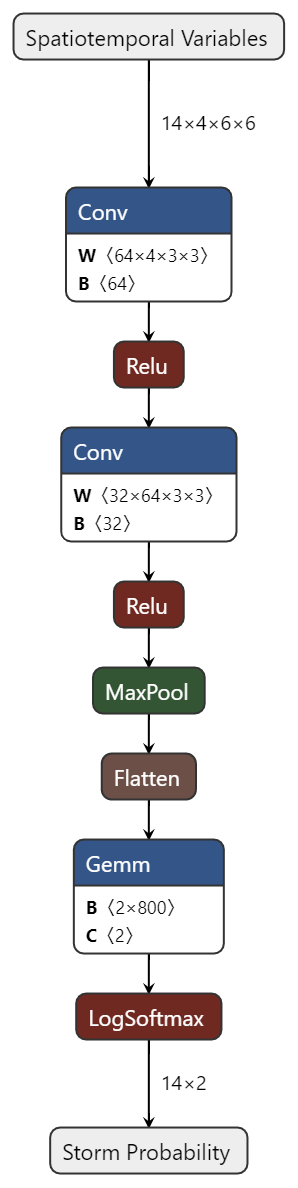
\includegraphics[height=14cm, width=0.48\linewidth]{pics/model.png}
    \caption{Visualized Architecture of CNN}
    \label{fig:CNN_fig}
\end{figure}

Essentially, Eq.~\ref{eq:cnn_prob}frames our task as a classification problem where the model predicts the probability of a high-wind event $(y_{ij})_t = 1$ based on local climate conditions $(\mathcal{O}^w_{ij})_t$. By applying this process, illustrated in Fig.~\ref{fig:example_CNN_pred}, across an entire geographical area, the CNN transforms the multi-channel climate input into a single-channel output: a map of storm probabilities. This concept of generating pixel-level predictions is central to many spatial deep learning models~\cite{van2016pixel}. % For practical applications, this continuous probability map can be converted into a discrete binary map of storm risk (0 = no storm, 1 = storm) by applying a decision threshold, such as 0.5.

 % Moreover, one can take a step back and view the whole pipeline as a pixel-to-pixel model \cite{van2016pixel}, i.e., CNN builds a spatiotemporal distribution of extreme wind speed over the pixels provided. 
 
\begin{figure}[h!]
    \centering
    \captionsetup{justification=centering}
    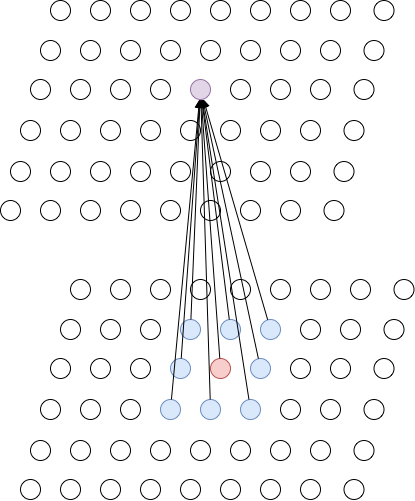
\includegraphics[width=\linewidth]{pics/pixtopix.png}
    \caption{An example of CNN prediction for $(\mathcal{O}^w_{ij})_t$. Here central pixel $i, j$ is in red, neighboring pixels of $(\mathcal{O}^w_{ij})_t$ are in blue, and output probability on the resulting map is in purple}
    \label{fig:example_CNN_pred}
\end{figure}

\subsubsection{Model Training}
\label{sec:training_val}

\paragraph{Dataset construction.}
Following Section~\ref{sec:data_collection_preprocessing}, each training sample consists of a local spatiotemporal patch of CMIP6 fields centred on a weather station pixel, paired with the binary storm label defined in Eq.~\ref{eq:target}. Formally, the dataset is
\begin{equation}
    \mathcal{D} = \left\{ \left(\mathcal{O}^w_{ij}\right)_t,\; (y_{ij})_t \right\}_{n=1}^{N_{\mathcal{D}}},
\end{equation}
where $N_{\mathcal{D}} = |\mathcal{S}_{\mathcal{D}}| \times T$ with $|\mathcal{S}_{\mathcal{D}}|$ the number of station-occupied pixels and $T$ the number of valid time steps after alignment. Each input patch has shape $C \times \Delta_t \times (2w{+}1) \times (2w{+}1)$, with $C=4$ channels (three CMIP6 variables: precipitation \texttt{pr}, maximum temperature \texttt{tasmax}, minimum temperature \texttt{tasmin}; plus static elevation---see ablation study in Section~\ref{sec:experiments}), temporal window $\Delta_t = 27$ days, and spatial half-width $w = 47$ pixels ($95 \times 95$ grid cells, covering roughly $106^\circ \times 106^\circ$ at the equator).

\paragraph{Train / validation / test split.}
The dataset is divided chronologically to prevent temporal leakage: \textbf{training} covers 2000-01-01 to 2020-12-31, \textbf{validation} 2021-01-01 to 2022-12-31, and \textbf{test} 2023-01-01 to 2024-12-31. All stations are present in every split; only the time axis differs. The validation set is used exclusively for early stopping (monitoring validation loss with patience of 10 epochs); no hyperparameter search is performed on it. Empirically, validation loss and Average Precision are well-correlated across epochs, so the best checkpoint by validation loss also yields near-optimal AP. This strict temporal separation ensures that the model is evaluated on conditions genuinely unseen during training.

\paragraph{Training protocol.}
The network is trained with the AdamW optimiser~\cite{https://doi.org/10.48550/arxiv.1412.6980} (learning rate $\eta = 10^{-4}$, weight decay $\lambda = 10^{-2}$) under a cosine annealing schedule that decays $\eta$ to $\eta/100$ over $T_{\max} = 20$ epochs. The loss is binary cross-entropy with logits and label smoothing $\varepsilon = 0.05$, which replaces hard targets $\{0,1\}$ with soft targets $\{0.05,\, 0.95\}$ and acts as a calibration regulariser~\cite{muller2019does}.

\paragraph{Class-imbalance handling via per-epoch resampling.}
The raw training set is heavily imbalanced: roughly 25\% of samples carry a positive label. A naive positive-class weight applied to the loss function can bias gradient updates and leads to poor calibration. We instead apply random undersampling at a 1:1 ratio, retaining all positive samples and an equal number of randomly selected negatives, reducing the training set from $\sim$3.1M to $\sim$1.4M samples. Crucially, the negative subsample is \emph{redrawn at the start of every epoch} using a fresh random seed (seed\,$=$\,epoch index), so the model encounters a different set of negative examples in each pass. Over $E$ training epochs this exposes the network to approximately $E$ times more unique negative examples than a fixed-subsample approach would, substantially reducing memorisation of a fixed training set. Preliminary experiments with a fixed subsample exhibited overfitting already by epoch~12; per-epoch resampling extended productive training to epoch~28 with consistent improvement in validation Average Precision (Figure~\ref{fig:train_val_ap}).

Training is distributed across two NVIDIA RTX A5000 GPUs (24~GB each) using PyTorch DDP with \texttt{fp16} mixed-precision arithmetic~\cite{paszke2019pytorch}. Each epoch processes 5{,}000 mini-batches of size 32. The model checkpoint with the highest validation Average Precision is selected for final evaluation.

\begin{figure}[t]
    \centering
    % Replace with actual plot: training AP and validation AP vs. epoch
    % fixed-subsample run (overfit at ep.12) vs. per-epoch-resample run (ep.28)
    \includegraphics[width=\linewidth]{pics/train_val_ap.png}
    \caption{Training and validation Average Precision across epochs for the fixed-subsample baseline (dashed) and the per-epoch resampling strategy (solid). Fixed subsampling causes validation AP to plateau and decline after epoch~12; per-epoch resampling sustains improvement through epoch~28.}
    \label{fig:train_val_ap}
\end{figure}

\paragraph{Evaluation metrics.}
Because storm events are rare (\textasciitilde42\% positive rate after 28-day aggregation), ranking-based metrics are more informative than accuracy. We report:
\begin{itemize}
    \item \textbf{AUROC} --- area under the receiver operating characteristic curve; measures overall discriminative ability independent of threshold.
    \item \textbf{Average Precision (AP)} --- area under the precision--recall curve; sensitive to the quality of positive-class detection.
    \item \textbf{F1, Precision, Recall} --- computed at the decision threshold of $p = 0.5$.
\end{itemize}
All metrics are computed both globally on the test set and stratified by geographic region and meteorological season (DJF, MAM, JJA, SON).


\section{Numerical Experiments}
\label{sec:experiments}
\subsection{Experimental Setup}

\paragraph{Hardware and reproducibility.}
All experiments are conducted on a server equipped with two NVIDIA RTX A5000 GPUs (24~GB VRAM each), 256~GB RAM, and 32 CPU cores. Training uses PyTorch~\cite{paszke2019pytorch} with the PyTorch Lightning framework and \texttt{fp16} mixed precision. Experiments are tracked with MLflow; model checkpoints are saved after every epoch and the best checkpoint by validation loss is used for final evaluation. The code and configuration files are available at \textcolor{brown}{[repository URL]}.

\subsection{Global Evaluation}

The model is trained on 6{,}045 GSOD stations worldwide over the period 2000--2020 using CMIP6 MRI-ESM2-0 as the climate input. Table~\ref{tab:metrics} reports the performance on the held-out test period (2023--2024).

\begin{table}[t]
    \centering
    \captionsetup{justification=centering}
    \begin{tabular}{l|c|c|c|c}
         \toprule
         Method & AUROC & AP & F1 & BSS \\
         \midrule
         CMIP threshold baseline  & 	extcolor{brown}{TBD} & 	extcolor{brown}{TBD} & --- & 	extcolor{brown}{TBD} \
         Logistic regression & 	extcolor{brown}{TBD} & 	extcolor{brown}{TBD} & --- & 	extcolor{brown}{TBD} \
         \midrule
         	extbf{CNN (pr+tasmax+tasmin+elev)} & 	extbf{0.851} & 	extbf{0.757} & 	extbf{	extcolor{brown}{TBD}} & 	extbf{0.320} \
         \midrule
         \multicolumn{5}{l}{	extit{Ablation study}} \
         \midrule
         \quad + sfcWindmax & 0.847 & 0.750 & 	extcolor{brown}{TBD} & 0.321 \
         \quad $-$ elevation & 0.847 & 	extcolor{brown}{TBD} & 	extcolor{brown}{TBD} & 	extcolor{brown}{TBD} \
         \quad $-$ precipitation & 	extcolor{brown}{TBD} & 	extcolor{brown}{TBD} & 	extcolor{brown}{TBD} & 	extcolor{brown}{TBD} \
         \quad $-$ temperature & 	extcolor{brown}{TBD} & 	extcolor{brown}{TBD} & 	extcolor{brown}{TBD} & 	extcolor{brown}{TBD} \
         
